\section{Evidence Response Signature}\label{sec:ers}

A risk estimator for \NDO{} verdicts can be wrong in ways that an aggregate metric such as log loss does not reveal. An estimator that lowers its risk when meaningless inputs are added, or that stays reassuring when the evidence has been tampered with, is unfit for purpose even if it scores well on one dataset. The Evidence Response Signature (\ers{}) states such requirements as properties with executable pass criteria. Conceptually, it applies the idea of metamorphic testing~\cite{chen2018metamorphic,segura2016survey} to the risk estimator rather than to the program. A transformation of the input evidence with a known expected effect on the output risk replaces an oracle for the risk itself, which is unavailable without adjudication.

\subsection{Properties, Perturbations and Pass Criteria}
Fig.~\ref{fig:ersframework} maps the eight properties to the perturbations that test them. Table~\ref{tab:ersprops} gives, for each property, its formal intent, the transformation, the pass and failure conditions as implemented in \code{sbgv8/ers.py}, the existing evidence and the main limitation. Table~\ref{tab:perturb} defines the perturbations operationally. The properties fall into three classes:
\begin{itemize}
\item \emph{Invariances} (negative controls; Properties 1 and 2): a correct estimator must not respond. They encode the principle that evidence \emph{quantity} is not evidence \emph{quality}.
\item \emph{Monotone requirements} (robustness tests; Properties 3, 4, 6, 8 and the environment check): degrading the evidence must not lower the risk. A move to abstention counts as a pass, because withdrawing a reassuring verdict when evidence weakens is correct behaviour.
\item \emph{Prescribed outcomes} (positive controls; Properties 5 and 7): the procedure must respond in a fixed way.
\end{itemize}
Formally, write $v_0=V(\Ev)$, $v_1=V(T_j(\Ev))$ and $\Delta=\Delta_j(\Ev)$, with tolerances $\epsilon=10^{-6}$ and $\delta=0.02$.

\begin{definition}[\ers{} conformance]\label{def:ers}
A trial of perturbation $T_j$ on an applicable record $\Ev$ \emph{passes} if
\begin{itemize}
\item invariance ($j\in\{\mathrm{P2},\mathrm{P3}\}$): $|\Delta|\le\delta\wedge v_1=v_0$;
\item monotone ($j\in\mathcal{M}$): $\Delta\ge-\epsilon\vee v_1=\INS{}$, applicable only if $v_0\neq\DIV{}$;
\item divergence ($j=\mathrm{P6}$): $v_1\in\{\DIV{},\INS{}\}\vee\Delta>0$;
\item integrity ($j=\mathrm{P8}$): $\iota(T_j(\Ev))=0\wedge v_1=\INS{}$,
\end{itemize}
where $\mathcal{M}=\{\mathrm{P1},\mathrm{P1b},\mathrm{P4},\mathrm{P5},\mathrm{P7},\mathrm{P9}\}$; a monotone trial with $v_0=\DIV{}$ is N/A. The \emph{conformance rate} of property $j$ on a corpus is passes divided by applicable trials. Its \emph{abstention credit} is the share of passes in which $v_1=\INS{}$ while the risk condition alone fails.
\end{definition}
The definition is a direct transcription of \code{ers.\_eval}. By Proposition~\ref{prop:indep}, a conformance rate of 1 says nothing about accuracy, and accuracy says nothing about the conformance rate; Remark~\ref{rem:vacuous} explains why abstention credit must be reported.

A trial whose perturbation cannot be applied is N/A and never counts as a pass. A monotone trial on a record that is already \DIV{} is N/A, because assurance risk is undefined there. Remark~\ref{rem:vacuous} applies throughout: passes are necessary, not sufficient, so we report abstention credit separately.

\begin{figure*}[!t]
\centering
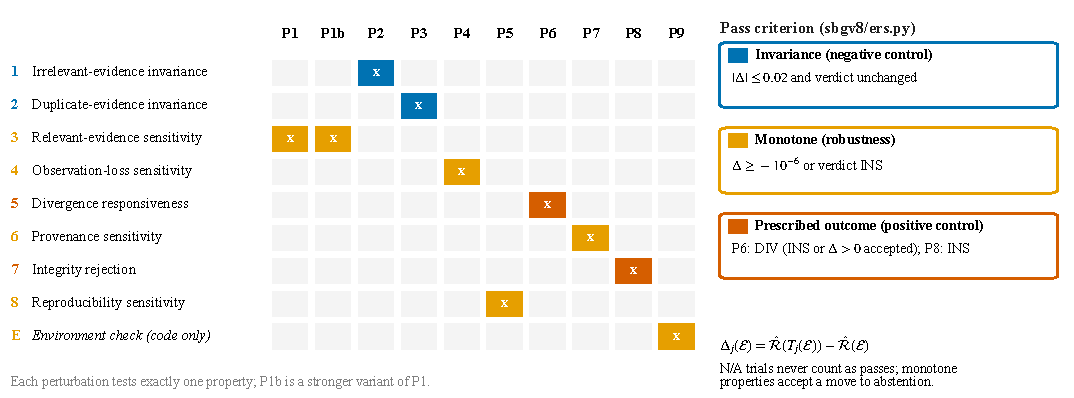
\includegraphics[width=\textwidth]{figures/fig_ers_framework.pdf}
\caption{\ers{} framework: the eight properties (rows; ``E'' is the environment check added by the implementation), the perturbation that tests each property (columns), and the three pass criteria (right), coloured by class. Each perturbation tests exactly one property.}
\label{fig:ersframework}
\end{figure*}

\begin{table*}[!t]
\caption{\ers{} properties: intent, transformation, pass and failure conditions as implemented (tolerances from \code{sbgv8/ers.py}: $10^{-6}$ for monotone properties, $0.02$ for invariances), existing evidence on the 312 development records, and limitations. ``Resp.'' counts applicable trials in which the fitted model's risk moved by more than the tolerance.}
\label{tab:ersprops}
\centering
\scriptsize
\setlength{\tabcolsep}{2.6pt}
\begin{tabular}{|c|L{2.35cm}|L{2.35cm}|c|L{2.1cm}|L{2.0cm}|L{3.3cm}|L{2.35cm}|}
\hline
\# & Property and formal intent & Transformation & $T_j$ & Pass & Failure & Existing evidence & Limitation \\
\hline
1 & Irrelevant-evidence invariance: $h(i)\cap U_c=\emptyset\Rightarrow$ no effect & Append inputs that hit only unchanged lines, fresh fingerprints & P2 & $|\Delta|\le0.02$ and $V$ unchanged & Risk moves or verdict changes & Probe failed 109/227 before the profile fix, 227/227 after; real-execution analogue: probe failed 5 of 7 & Appended records are synthetic; two inputs per trial \\
2 & Duplicate-evidence invariance: copies add no information & Append two flagged copies of existing inputs & P3 & as P2 & as P2 & All predictors 262/262 & Flagged copies only; unflagged copies are handled by the fix, not tested here \\
3 & Relevant-evidence sensitivity: removing sole support may not lower risk & Delete a sole reacher of a changed unit (P1); all covers of the least-multiplicity unit (P1b) & P1, P1b & $\Delta\ge-10^{-6}$ or $V{=}\INS{}$ & Risk falls & All pass (16, 93); fitted model Resp.\ 9/16, 68/93 & P1 applicable to only 16 records \\
4 & Observation-loss sensitivity: fewer channels may not lower risk & Remove one captured channel from every input & P4 & as P1 & Risk falls & All pass (178); Resp.\ 0 & Fitted model is indifferent, so the pass is vacuous for it \\
5 & Divergence responsiveness: a witness withdraws \NDO{} & Append a confirmed-difference input hitting all changed units & P6 & $V{=}\DIV{}$; \INS{} or $\Delta>0$ accepted & \NDO{} kept with $\Delta\le0$ & Recorded V7-B failed 71 (157 passes are abstention credit); recomputed and \sbg{} 228/228 & Synthetic witness; real-execution analogue applicable once \\
6 & Provenance sensitivity: weaker provenance may not lower risk & Mark all inputs label-derived & P7 & as P1 & Risk falls & All pass (178); Resp.\ 0 & \code{prov\_ok} constant in training \\
7 & Integrity rejection: violation forces abstention & Set $\iota(\Ev)=0$ & P8 & $V{=}\INS{}$ & Any other verdict & Recorded V7-B failed 155, recomputed V7-B 84 (all \DIV{}); \sbg{} 312/312 & Tests the decision procedure; passes by construction under the trust gate \\
8 & Reproducibility sensitivity: less determinism may not lower risk & Mark half the deterministic inputs non-deterministic; halve repeats & P5 & as P1 & Risk falls & All pass (176); Resp.\ 100/176; real-execution analogue 30/30 for all predictors & Repeated deterministic runs are not independent samples \\
E & Environment check: inconsistency may not lower risk & Mark environment inconsistent & P9 & as P1 & Risk falls & All pass (228); Resp.\ 0 & \code{env\_ok} constant in training \\
\hline
\end{tabular}
\end{table*}

\begin{table}[!t]
\caption{Controlled evidence perturbations (\code{sbgv8/perturb.py}). Ctrl.: N negative control, P positive control, R robustness (monotone). Mode: H = post-hoc edit of a record copy (all ten, evaluated on 312 records); X = an execution-level analogue also exists (30 pairs, macOS, exploratory). App.: applicable trials of 312.}
\label{tab:perturb}
\centering
\scriptsize
\setlength{\tabcolsep}{2.4pt}
\begin{tabular}{|c|L{3.55cm}|c|c|c|r|}
\hline
Id & Operation & Prop. & Ctrl. & Mode & App. \\
\hline
P1 & Delete one clean input that is the sole reacher of a changed unit or sole capturer of a channel & 3 & R & H & 16 \\
P1b & Delete all clean inputs covering the least-multiplicity unit & 3 & R & H & 93 \\
P2 & Append two \code{SAME} inputs hitting only unchanged lines & 1 & N & H, X & 227 \\
P3 & Append two flagged copies of existing inputs & 2 & N & H & 262 \\
P4 & Remove one captured channel from every input & 4 & R & H & 178 \\
P5 & Mark half of deterministic \code{SAME} inputs non-deterministic; halve repeats & 8 & R & H, X & 176 \\
P6 & Append a confirmed-difference witness hitting all changed units & 5 & P & H, X & 228 \\
P7 & Mark the provenance of all inputs label-derived & 6 & R & H & 178 \\
P8 & Set the integrity flag to violated & 7 & P & H & 312 \\
P9 & Mark the execution environment inconsistent & E & R & H & 228 \\
\hline
\end{tabular}
\end{table}

\begin{algorithm}[!t]
\caption{\ers{} evaluation of one trial}
\label{alg:ers}
\small
\begin{algorithmic}[1]
\Statex \textit{Implements:} \bcode{ers.compute\_ers}, \bcode{ers.\_eval}
\Require record $\Ev$, predictor $(\Rhat,V)$, perturbation $j$, seed
\State $(\Ev',\mathit{applicable})\gets T_j(\textsc{copy}(\Ev))$ \Comment{the sealed evidence is never modified}
\If{\textbf{not} $\mathit{applicable}$} \Return N/A \EndIf
\State $\Delta\gets\Rhat(\Ev')-\Rhat(\Ev)$;\ $v_0\gets V(\Ev)$;\ $v_1\gets V(\Ev')$
\If{$j$ is monotone (P1, P1b, P4, P5, P7, P9)}
  \If{$v_0=\DIV{}$} \Return N/A \EndIf
  \State \Return pass iff $\Delta\ge-10^{-6}$ \textbf{or} $v_1=\INS{}$
\ElsIf{$j\in\{$P2, P3$\}$} \Return pass iff $|\Delta|\le0.02$ \textbf{and} $v_0=v_1$
\ElsIf{$j=$ P6} \Return pass iff $v_1=\DIV{}$ \textbf{or} $\Delta>0$ \textbf{or} $v_1=\INS{}$
\Else{} \Return pass iff $\iota(\Ev')=0$ \textbf{and} $v_1=\INS{}$ \Comment{P8}
\EndIf
\end{algorithmic}
\end{algorithm}

\subsection{Post-Hoc and Execution-Level Perturbations}
Table~\ref{tab:perturb} gives each perturbation's mode. All ten, as evaluated on the full corpus, are \emph{post-hoc transformations}: they edit a copy of the record an execution produced and re-execute nothing. That makes them cheap, deterministic and exactly repeatable, and it is the right instrument for testing how an \emph{estimator} responds to its input. It is the wrong instrument for estimating how a \emph{program} or the \emph{collector} would behave under the corresponding real change. A post-hoc P2 record claims to reach only unchanged lines, whereas a real irrelevant input could have side effects. We therefore read $\Delta_j$ as a description of the estimator, never as a causal effect.


\paragraph*{Execution-level analogues} For P2, P5 and P6, an execution-level analogue re-runs the collector with changed conditions. P2 adds real inputs that exercise only unchanged code. P5 re-runs with fewer repetitions. P6 adds a discriminating input found by a seeded generator that never sees outputs or labels. These analogues were run once, on macOS, on 20 development pairs selected by a rule declared and stored before any run (seeded quotas per arm, no labels used), plus a supplementary cohort of 10 pairs with $Y{=}1$. The supplementary cohort was declared after the primary run showed P6 applicable on none of the 20 pairs, and we report it separately for that reason. The run used the pre-fix profile from a working tree with uncommitted modifications (recorded in its manifest). Its per-trial results (720 rows) are preserved, but its per-run evidence directories are not, so we treat it as exploratory corroboration (Section~\ref{sec:res-rq2}).

\subsection{Two Roles of the Signature}
\ers{} plays two roles in \sbg{}, which we evaluate separately.
\begin{itemize}
\item As a \emph{conformance test}, the property matrix checks whether an estimator and decision procedure satisfy the properties on real evidence records. This role uses no labels (RQ2).
\item As \emph{predictive features}, the responses $\Delta_j$ are appended to the profile in the full \cec{} model. The hypothesis is that how strongly an estimate reacts to evidence degradation carries information about risk beyond the profile itself. This role is evaluated by matched-coverage risk and proper scoring rules against labels (RQ4).
\end{itemize}
